\documentclass{article}
\usepackage{geometry}
\usepackage{graphicx}
\usepackage{amsmath}
\usepackage{algorithm}
\usepackage{algpseudocode}
\usepackage{makeidx}

\makeindex

\geometry{
a4paper,
top=10mm,
bottom=15mm,
left=10mm,
right=10mm,	
}

\begin{document}

\pagenumbering{gobble}
\newgeometry{
top=30mm,
bottom=50mm,
left=20mm,
right=20mm,
}

\begin{center}

\textbf{\Huge Binary Search} \\
\vspace{50pt}
{\large An Article for Assignment 6 on \LaTeX } \\
\textbf{\large CS251: Computer Laboratory} \\
\vspace{100pt}

\textbf{\large Jayant Agrawal} \\
(14282)
\vspace{30pt}

INSTRUCTOR \\
\textbf{Prof. Arnab Bhattacharya}
\vspace{100pt}


\includegraphics[width=0.3\columnwidth]{logo.jpg}\\
\textbf{\large Department of Comuter Science and Engineering \\
INDIAN INSTITUTE OF TECHNOLOGY KANPUR \\
KANPUR 208016, INDIA \\ } 
\vspace{20pt}
Feb 2016


\end{center}

\restoregeometry
\newpage
\pagenumbering{roman}
\tableofcontents
\addcontentsline{toc}{section}{\listfigurename}
\addcontentsline{toc}{section}{\listtablename}
\listoffigures
\listoftables


\newpage
\pagenumbering{arabic}

\section{Abstract}
Searching \index{Searching} and Sorting \index{Sorting} are the two most basic routines that are involved in almost every Software \index{Software}. As the name suggests, searching involves finding a key in a given list. The trivial solution is to iterate over all the elements of the list and report whether the key is found or not. The Time Complexity \index{Complexity} involved in this operation is of the order of the size of the list. In this article, we see how to solve this problem in a much more efficient way. The solution is known as \textbf{Binary Search} \index{Binary} and the time complexity involved is of the order of $log(n)$ , if the given input is arranged nicely, where 'n' is the size of the given list or set.


\section{Algorithm}
Though, this approach has a wide variety of applications, it is most commonly used to find a given value within a sorted sequence\index{sequence}.
It works by repeatedly dividing in half the portion of the list that could contain the item, until you've narrowed down the possible locations to just one.\cite{khan} \\

The main idea of binary search is to keep track of reasonable guesses. Lets say that A and B are playing a game known as the \textit{guessing game}, where A selects a number between 1 and 100.
Now, B's job is to find out the number that A selected. Lets say B comes up with two guesses, 25 and 81. A says that his number is higher than the first guess and lower than the second guess.

\begin{figure}[h!]
\begin{center}
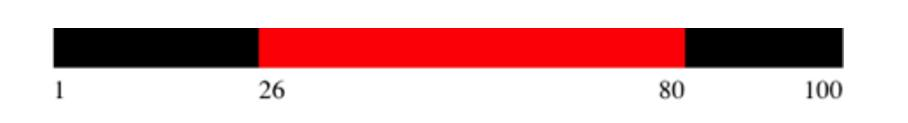
\includegraphics[width=0.5\columnwidth]{one1.jpg}
\caption{Red Area : Reasonable guesses}
\label{fig:one}
\end{center}
\end{figure}

Then, it is obvious that the selected number lies between 26 and 80. Figure \ref{fig:one} shows the remaining area of reasonable guesses. We can safely ignore the black region.
In the next turn, it is reasonable to guess a number such that it divides the set of reasonable guesses into two ranges of the same size. If the guess is not correct, then based on A's response whether the guess is too high or low, we can again discard half the remaining choices. 
For example, in this case the halfway point would be $(26+80)/2$, or 53. If A says that it is too high, then we can eliminate 53 to 80 as shown in Figure \ref{fig:two}.
\begin{figure}[h!]
\begin{center}
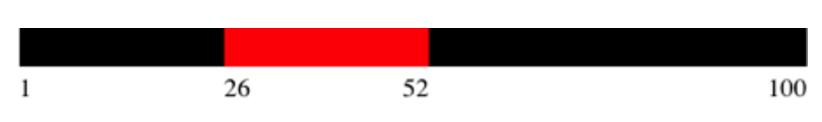
\includegraphics[width=0.47\columnwidth]{two2.jpg}
\caption{Remaining set of guesses}
\label{fig:two}
\end{center}
\end{figure}

In this way we can keep halving the size or our domain and arrive at the correct guess.
We can formulate our \index{algorithm}algorithm as follows. Let the variable $left$ be the correct minimum reasonable guess, and $right$ be the correct maximum reasonable guess. The input to the problem is the number $n$, the highest possible number that the opponent can think of. We assume that the lowest possible number that can be chosen is 1. The algorithm is as follows. \cite{khan}

\begin{itemize}
\item Let $left = 1$ and $right=n$.
\item Guess the average of $right$ and $left$, rounded down (so that it is an integer).
\item If you guesses the number, $stop$ . You found it!.
\item If the guess was too low, set $left$ to be one larger than the guess.
\item If the guess was too high, set $right$ to be one smaller than the guess.
\item Go back to step 2.
\end{itemize}

Following is the pseudo code for the above algorithm.
\subsection{Pseudo-Code}
Consider the simple problem of finding a \index{key}key within an \index{array}array. The following pseudo-code returns the \index{index}index of the key, if it is found. Let the size of the array '$A$' be '$n$'. \cite{wiki}


\begin{algorithm}
\caption{Binary Search Algorithm}
\label{binalgo}
\begin{algorithmic}[1]
\Procedure{BinSearch}{}
\State $left \gets 0 $
\State $right \gets n-1 $
\While{ $right \leq left$ }
\State $mid \gets (left+right)/2 $
\If{ $A[mid] == key $ }
\State return $mid$
\ElsIf {$A[mid] < key $}  \Comment{\parbox[t]{.5\linewidth}}{Discarding left half} 
\State $left \gets mid + 1 $ 
\Else  \Comment{\parbox[t]{.5\linewidth}}{Discarding right half}
\State $right \gets mid - 1$
\EndIf
\EndWhile
\State return $NOT\_FOUND$
\EndProcedure
\end{algorithmic}
\end{algorithm}

\subsection{Complexity}
Consider Algorithm \ref{binalgo}, it is easily observable that each \index{iteration}iteration the set of remaining guesses reduces exactly by half untill there is only one value left.
At each iteration the time taken is of the order of \index{constant}constant time. So, the time complexity of our algorithm depends only on the number of total iterations. 
We start with the total size of $n$ and end up at the size of one irrespective of whether we find the key or not, after halving the size of the set at each iteration.
Thus, the total no of iterations are of the order of $log_2(n)$. \\
\begin{table}[h!]
\begin{center}
\begin{tabular}{|c|c|}
\hline
n & $log_2(n)$ \\
\hline
1 & 0 \\
2 & 1 \\
4 & 2 \\
8 & 3 \\
16 & 4 \\
32 & 5 \\
64 & 6 \\
128 & 7 \\
256 & 8 \\
512 & 9 \\
1024 & 10\\
1048576 & 20 \\
2097152 & 21 \\
\hline
\end{tabular}
\caption{No of Iterations for different values of $n$ }
\label{table:one}
\end{center}
\end{table}

Table \ref{table:one} shows the no of iterations it takes for different values of n. 
Therefore, assuming the RAM\index{RAM} model of computaion\index{computation}, the time complexty of the algorihtm $T_0(n)$ is given by:

\begin{align}
T_0(n) = O(log_2(n))
\label{eq:bin1}
\end{align}


\section{\index{Pre-Processing}Pre-Processing Time}
\label{sec:pre}
In the above description, we have always assumed that the given input is sorted.
If the given is sorted, then pre-processing time is of the order of constant time.
Binary Search should always be applied in this case. \\

Now, if the input is in a random order, binary search algorithm can not be applied without pre-processing.
For the algorithm to be applicable it is necessary that the input be sorted. So, the pre-processing time is equivalent to the time taken to sort the input.
The fastest sorting algorithm that exists, takes $O(n*log(n))$ time, where $n$ is the size of the given input.

\section{Comparison with \index{linear}linear search}

Table \ref{table:one} can also be shown as in Figure \ref{fig:two}. \\

\begin{figure}[h!]
\begin{center}
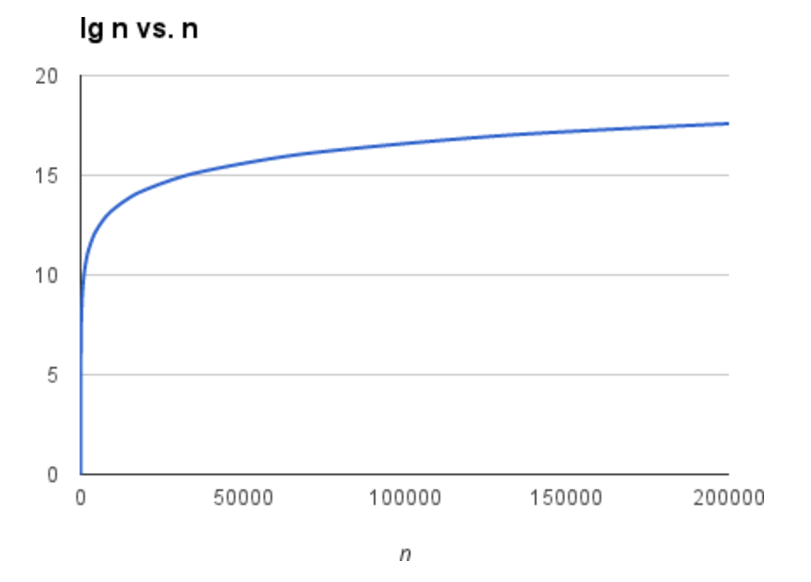
\includegraphics[width=0.47\columnwidth]{three.jpg}
\caption{ $log(n)$ vs $n$ }
\label{fig:two}
\end{center}
\end{figure}

\textbf{Linear Search} is a technique where the key is searched by going over the entire set of inputs and checking if the element is the key or not.
Obviously, the time taken for this algorithm in the worst case is of the order of the size of the input i.e. $n$ [$O(n)$].  \\

As mentioned in Section \ref{sec:pre}, if the given input is sorted, binary search should be applied irrespective of the input size and no of queries\index{queries}.
But if the given input is not sorted the deciding between binary search and linear search depends upon the application conditions.\\

Let the number of querries be $k$. Then, the total time taken for the Binary Search algorithm ($T_1(n)$) is given by :
\begin{align}
T_1(n) = O(n*log(n) + k*log(n))
\label{eq:bin2}
\end{align}

The total time taken for Linear Search Algorithm ($T_2(n)$) is given by :
\begin{align}
T_2(n) = O(k*n)
\label{eq:linear}
\end{align}

In the case of a single query, Equations \ref{eq:bin1} ,\ref{eq:bin2} and \ref{eq:linear} can be visualised as in Figure \ref{fig:time}.
\begin{figure}[h!]
\begin{center}
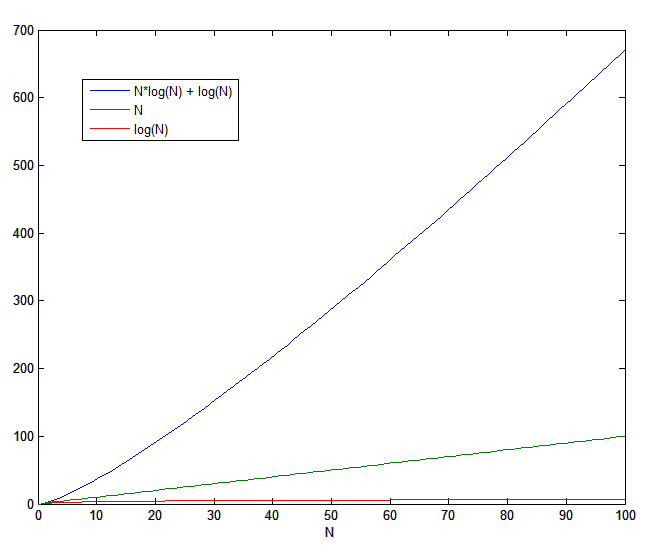
\includegraphics[width=0.47\columnwidth]{time.png}
\caption{ For k = 1, Single Query  }
\label{fig:time}
\end{center}
\end{figure}

\subsection{No of Queries- Large}
For large k, from Equations \ref{eq:bin2} and Equations \ref{eq:linear}, we can see that, we should apply binary search algorithm.
\subsection{No of Queries- Low}
In this case, the approach to be applied depends on the input size $n$. For small n, the time taken for both the approaches is similar.\\

\textbf{Note: }In some applications, we need to insert some elements in the input set and then search for the key. In the case of binary search algorithm, inserting takes extra time whereas in linear search inserting is easy.
Similarly for deletion. Thus, the approach to be applied depends on these parameters as well.

\subsection{Summary}
Table \ref{table:summary} summarizes the comparison between binary and linear search.

\begin{table}[h!]
\begin{center}
\begin{tabular}{|c|c|c|c|}
\hline
\textbf{Sr. No.} & \textbf{Comparison} & \textbf{Linear Search} & \textbf{Binary Search}\\
\hline
1 & Time Complexity & $O(n)$ & $O(log_2(n))$ \\
2 & Best Case time & $O(1)$ [First element] & $O(1)$ [Center element] \\
3 & Prerequisite [Array] & None & Sorted \\
4 & Worst Case[n=1000] & 1000 comparisons & 10 comparisons \\
5 & Data Structure & Array, Linked List & Array \\
6 & Insert Operation & Easy & Requires processing \\
\hline
\end{tabular}
\caption{Comparison between Linear search and Binary Search\cite{uni}}
\label{table:summary}
\end{center}
\end{table}

\section{Conclusion}
Binary search is a more efficient searching technique than linear search but insertion of an element is not efficient as it requires arranged elements in specific order. Further it is also possible to apply binary search on linked list by making necessary modifications to original binary search algorithm. The selectiom of searching algorithm can be based on the data structure on to which it is applied and which operations are required more. Balance is required between search and maintanance of a data structure.\cite{uni}


\addcontentsline{toc}{section}{References}
\bibliographystyle{alpha}
\bibliography{cse}
\newpage
\addcontentsline{toc}{section}{Index}
\printindex
\end{document}
